%% \documentclass[twocolumn]{article}
\documentclass[pre,twocolumn,twoside,byrevtex,superscriptaddress]{revtex4}

\usepackage{amsmath}
\usepackage{amssymb}
\usepackage{url}
\usepackage{graphicx}
\usepackage{listings,color}
\usepackage{setspace}

\lstset{language=matlab,
        basicstyle=\ttfamily\scriptsize\singlespacing,
        keywordstyle=\color{blue},
        stringstyle=\color{red},
        commentstyle=\color{green},
        morecomment=[l][\color{magenta}]{\#},
        frame=L,
        xleftmargin=\parindent,
        numbersep=5pt,
        breaklines=true,
        breakatwhitespace=false,
        escapeinside={\%*}{*)},
}

\setlength{\parindent}{0cm}

\setlength{\parskip}{1mm}

\begin{document}

%% \twocolumn[
%%   \begin{@twocolumnfalse} 

%%     \title{\vspace{-2cm}Homework 4: Counterprop}
%%     \author{Andy Reagan}

%%     \maketitle

%%   \end{@twocolumnfalse}
%% ]

\title{\vspace{-2cm}Homework 4: Counterprop}
\author{Andy Reagan}

\begin{abstract}
A basic version of the counterpropogation algorithm is coded up, and put through some simple tests.
I find that it performs best when training with Kohonen and Grossberg layers simulanteously, when the learned parameters are not scaled, and when run from random initial weights (as opposed to nearest neighbor).
\end{abstract}

\maketitle





\section{Introduction}

The original version of the counterpropogation algorithm was originally proposed by Neilson in 1988 \cite{hecht1987counterpropagation} with a later paper describing the applications \cite{hecht1988applications}.
Here I code up a version using the psuedocode from Rizzo and Doughtery's application to characterizing aquifer properties \cite{rizzo1994characterization}.

The main idea of counterpropogation is a combination of the classification power of Kohonen's map, with the interpolation ability of a Grossberg net.
Claimed advantages of counterpropogation are higher speed than backpropogation, and the ability to better recognize patterns.

As I have found to be the case with coding the nueral networks, there are many parameters and choices that are left up to the programmer.
In the next section we explore a few, namely: order of presentation of training data, effect of training the layers together or separate, on scaling the learning coefficients, and on initializing the weights.

\begin{figure}[h]
 \centering
  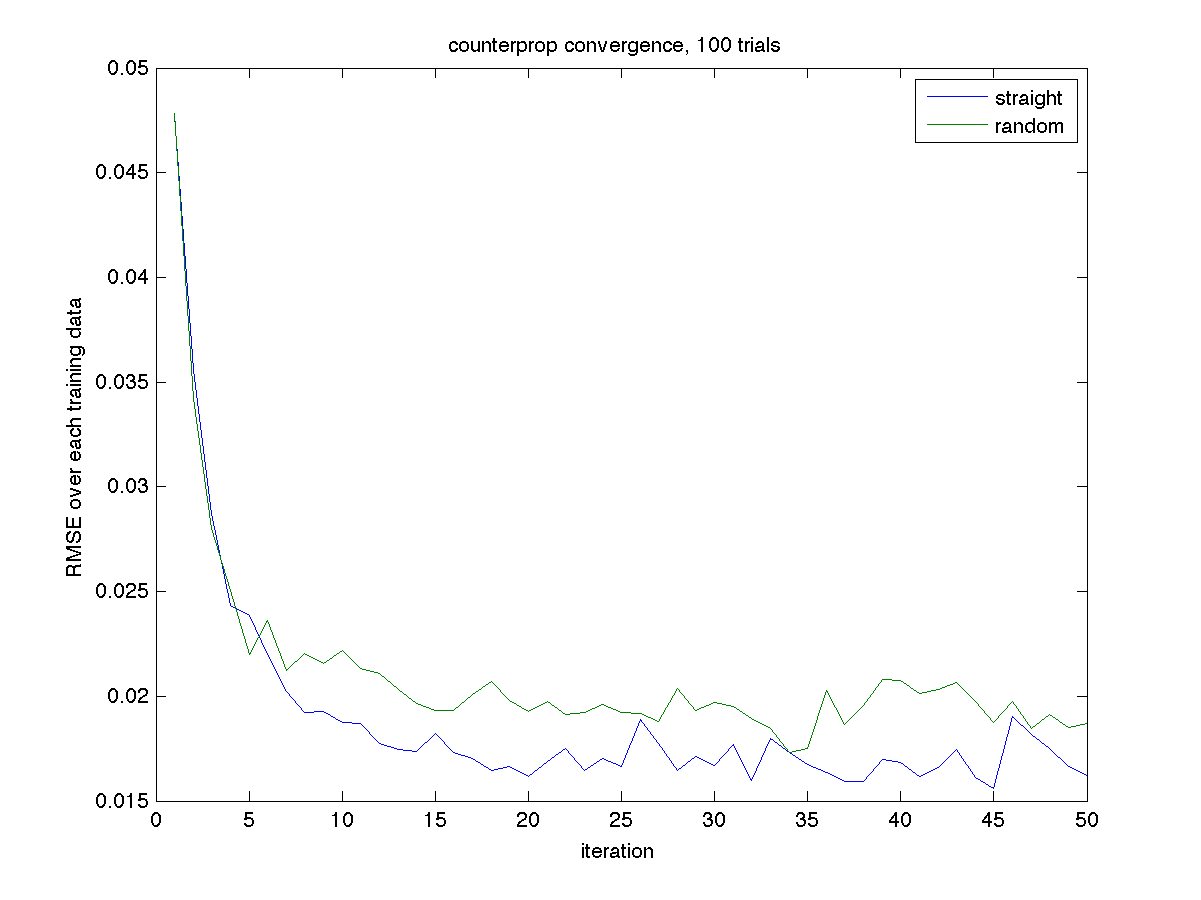
\includegraphics[width=0.48\textwidth]{115.png}
  \label{fig:5}
  \caption{Direct comparison over 100 trials of the convergence when presenting training data in a random or repeated order.}
\end{figure}

\begin{figure}[h]
 \centering
  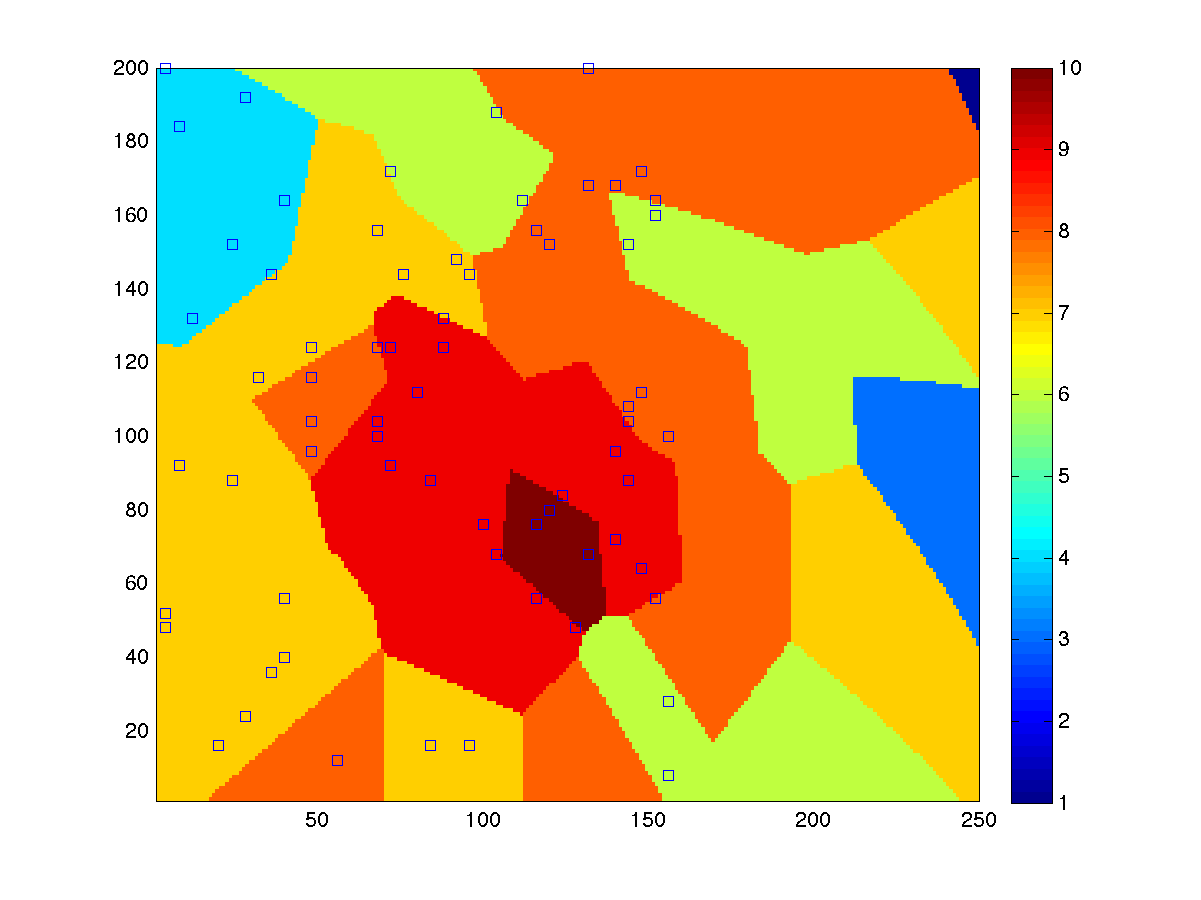
\includegraphics[width=0.48\textwidth]{116-wpoints.png}
  \label{fig:10}
  \caption{Classification of full data (interpolation phase), with points at where the training data were.}
\end{figure}

\section{Methods}

I code the network in MATLAB, again following the psuedocode from Rizzo and Doughtery \cite{rizzo1994characterization}.
Specific choices of parameters are investigated further.

I set the number of Kohonen nuerons to be 3 greater than the size of the training data when not using the network as a nearest-neighbor classifier.
This is such that the Kohonen vectors can be useful in a nearest-neighbor classification fashion, but without prior assumptions about the distributions of the given observations.
Another interesting thing to try would be to explicitly remove the Kohonen nodes whose input weights go to zero, and therefore use the Kohonen layer to reduce the data into clusters.
I don't expect that removing these nodes would have any effect, but it would be good to check.


\section{Results}

First, the main challenge of getting the network to run, and converge, was successful.
Both operating from a random initial condition on the weights on and on a preset nearest neighbor condition, we are able to make spatially reasonable predictions for the training data.

As an interpolater, the Grossberg layer classifies the ``fuzzy'' output of the Kohonen layer as a winner-takes-all, and this seems like a reasonable and simple way to classify this output.

I find that despite my expectations, the best convergence is achieved without scaling parameters.
The best performance is also achieved while training together, and agian best performance is achieved on initializing the weights randomly, and letting the Kohonen layer do it's thing.
Intiutively, as a spatial classifier, I really like counterpropogation.

Each of the following figures is the result of a test of each of these over 100 trials.
I apologize for the tiny font size, MATLAB default.


\begin{figure}[h]
 \centering
  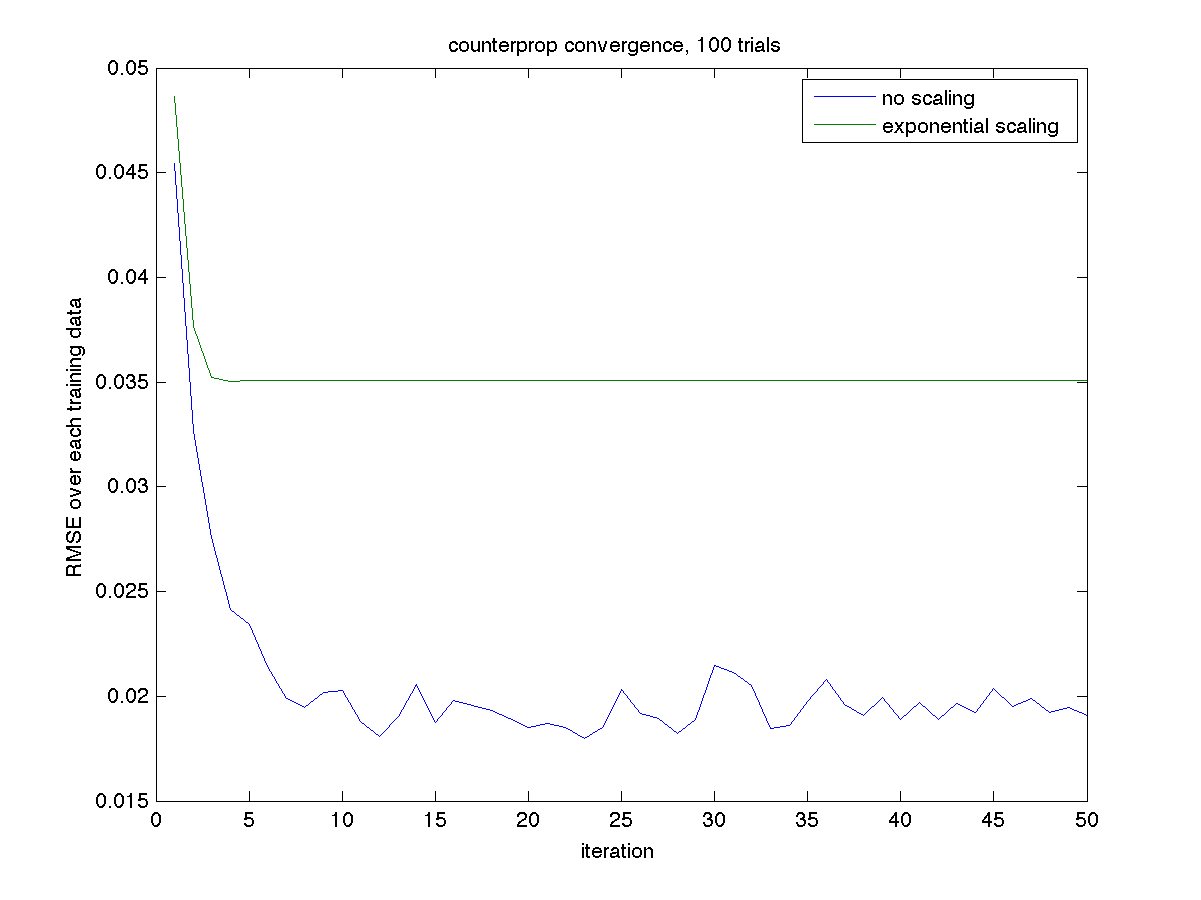
\includegraphics[width=0.48\textwidth]{117.png}
  \label{fig:7}
  \caption{Convergence with different scalings of learning parameters.}
\end{figure}

\begin{figure}[h]
 \centering
  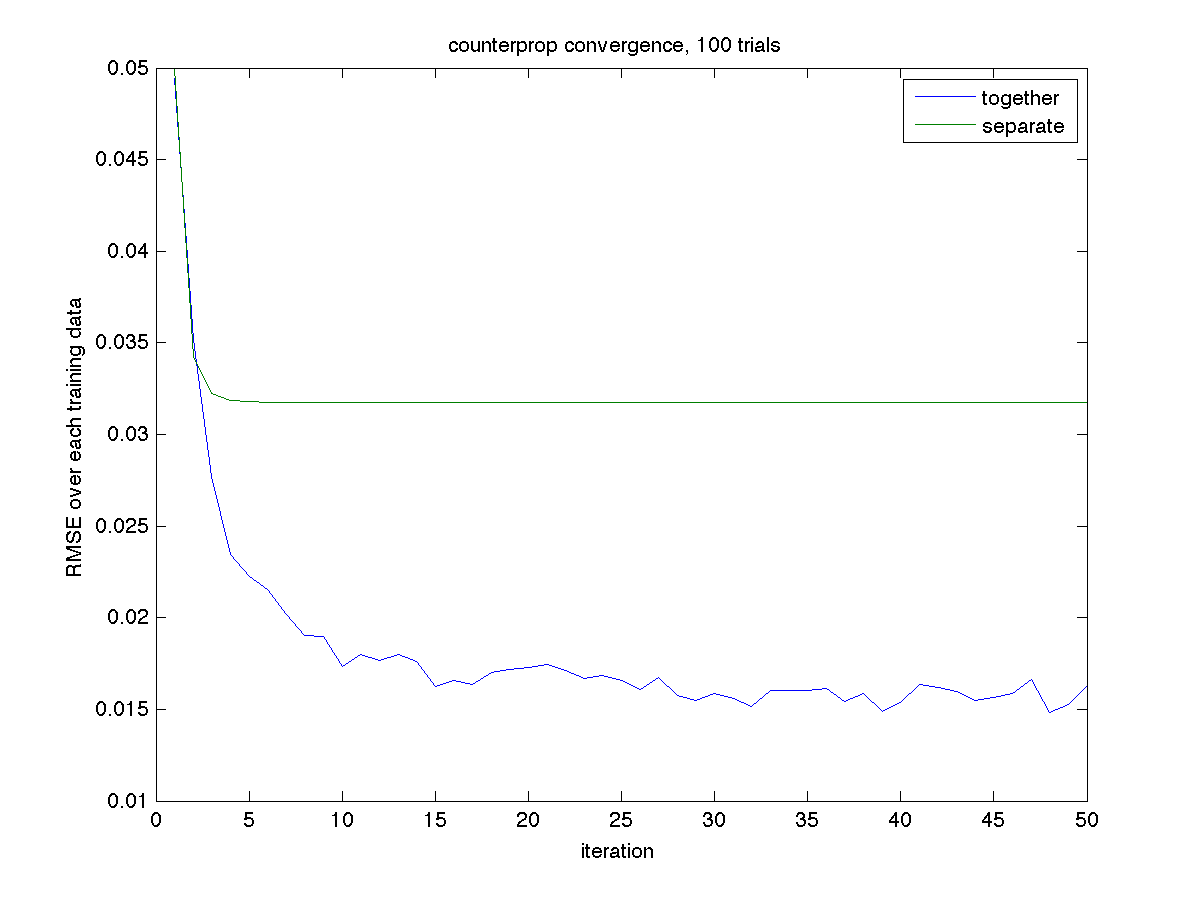
\includegraphics[width=0.48\textwidth]{118.png}
  \label{fig:8}
  \caption{Covergence training together and separate.}
\end{figure}

\begin{figure}[h]
 \centering
  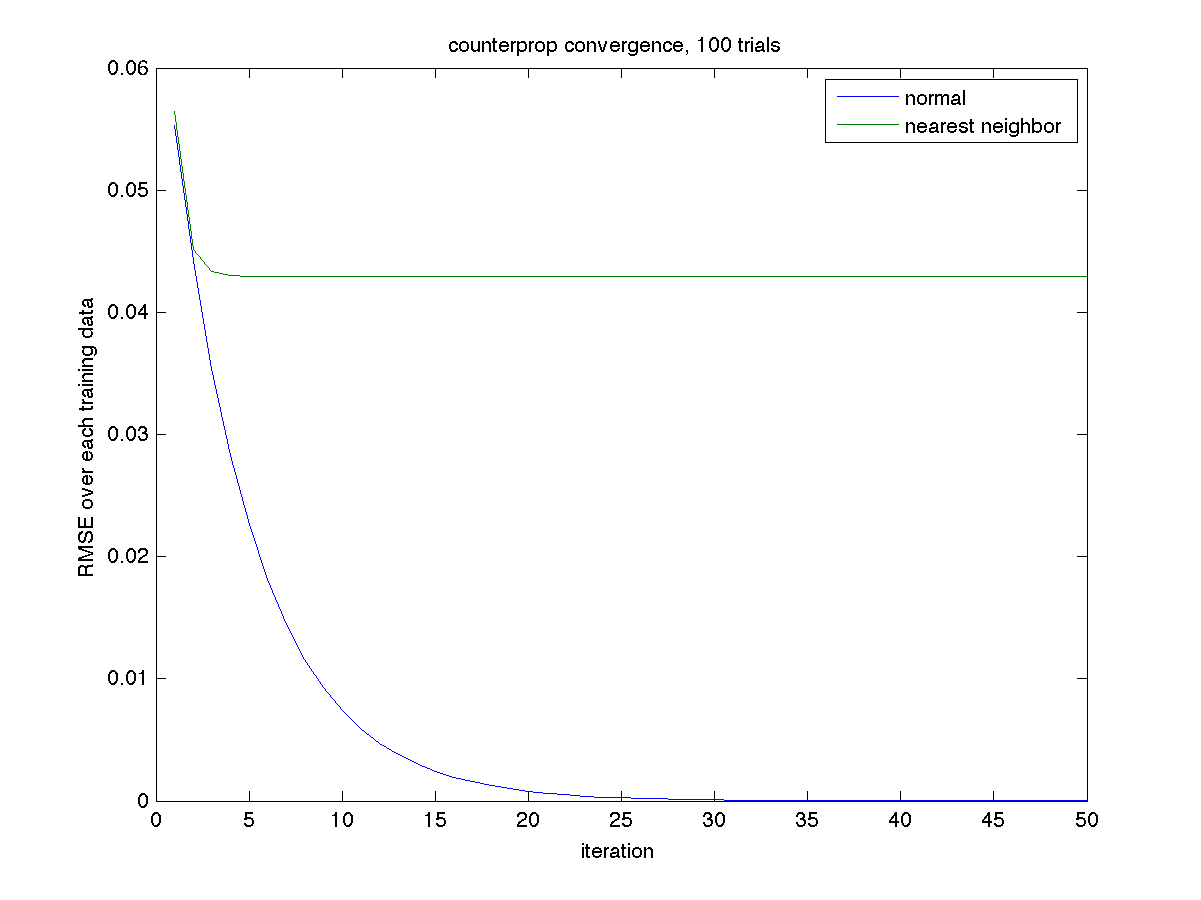
\includegraphics[width=0.48\textwidth]{119.png}
  \label{fig:9}
  \caption{Covergence with different Kohonen layer weight initializations.}
\end{figure}

\clearpage
\pagebreak

\bibliographystyle{chicago}
\bibliography{writeup}

\clearpage
\pagebreak
\onecolumngrid

    \section*{Full code}

    \lstinputlisting{counterprop_andy_driver.m}

    \lstinputlisting{nomalize_input_andy.m}

    \lstinputlisting{train_counterprop_andy.m}

    \lstinputlisting{test_counterprop_andy.m}

    \lstinputlisting{scaling_exponential.m}

    \lstinputlisting{scaling_none.m}

\clearpage
\pagebreak

    \section*{Extra figures}

    \begin{figure}
      \centering
      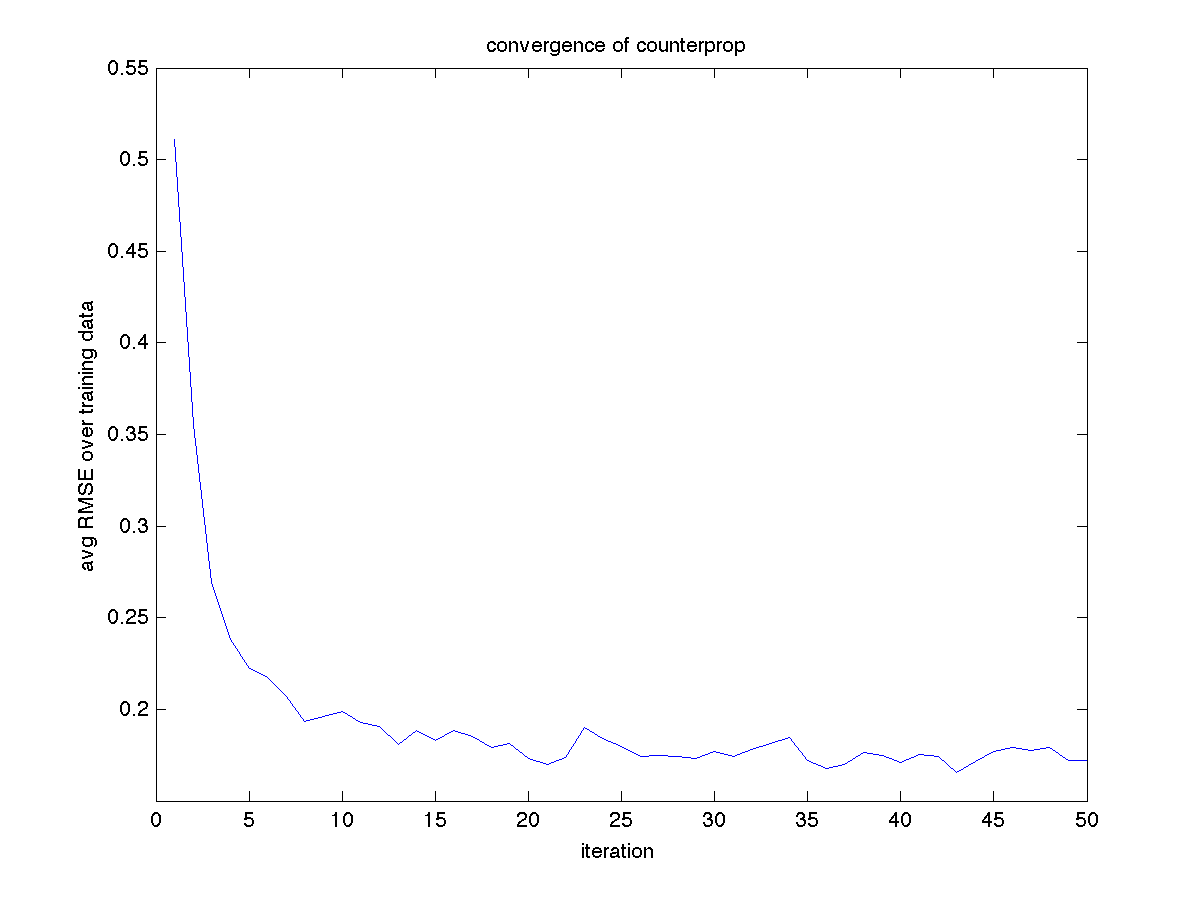
\includegraphics[width=0.68\textwidth]{111.png}
      \label{fig:1}
      \caption{Basic convergence test.}
    \end{figure}

    \begin{figure}
      \centering
      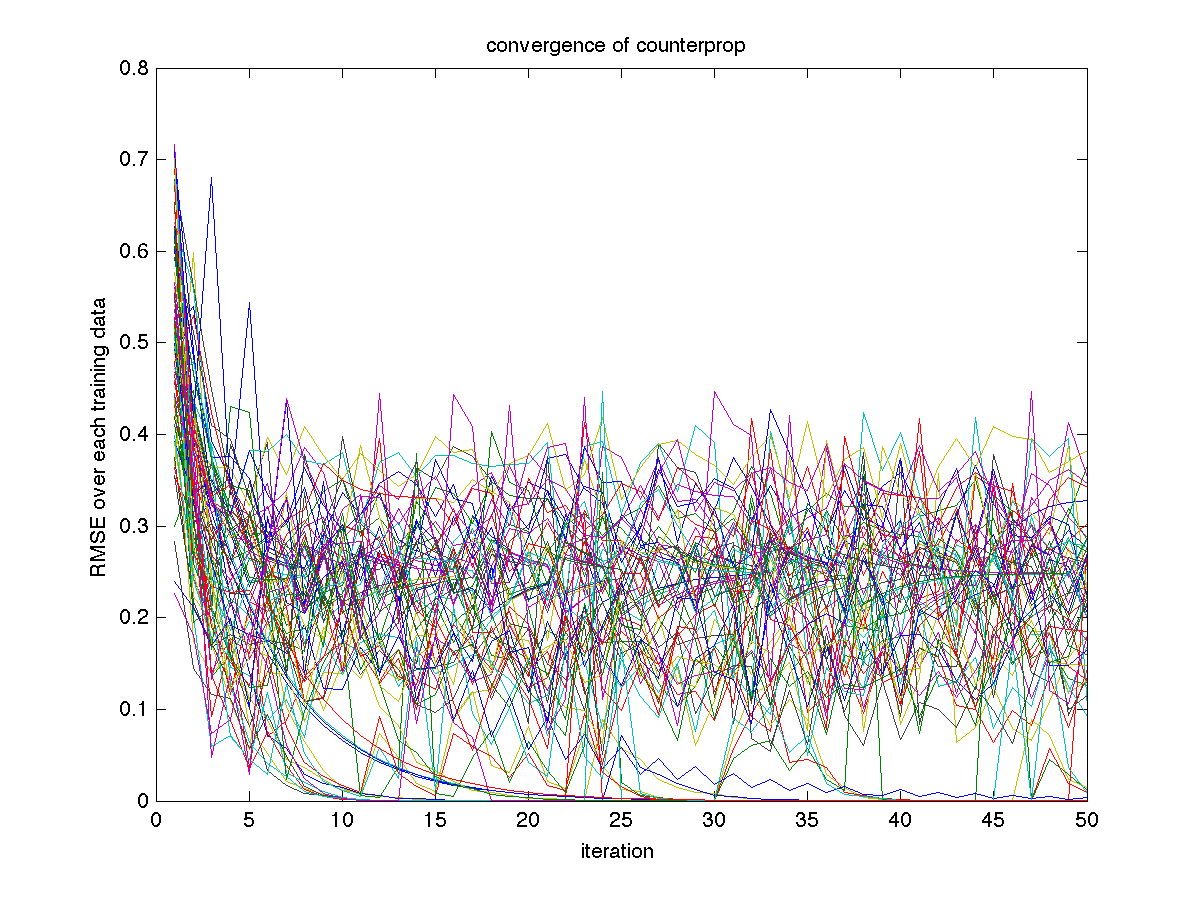
\includegraphics[width=0.68\textwidth]{112.png}
      \label{fig:2}
      \caption{Convergence on each of the individual training data.}
    \end{figure}

    \begin{figure}
      \centering
      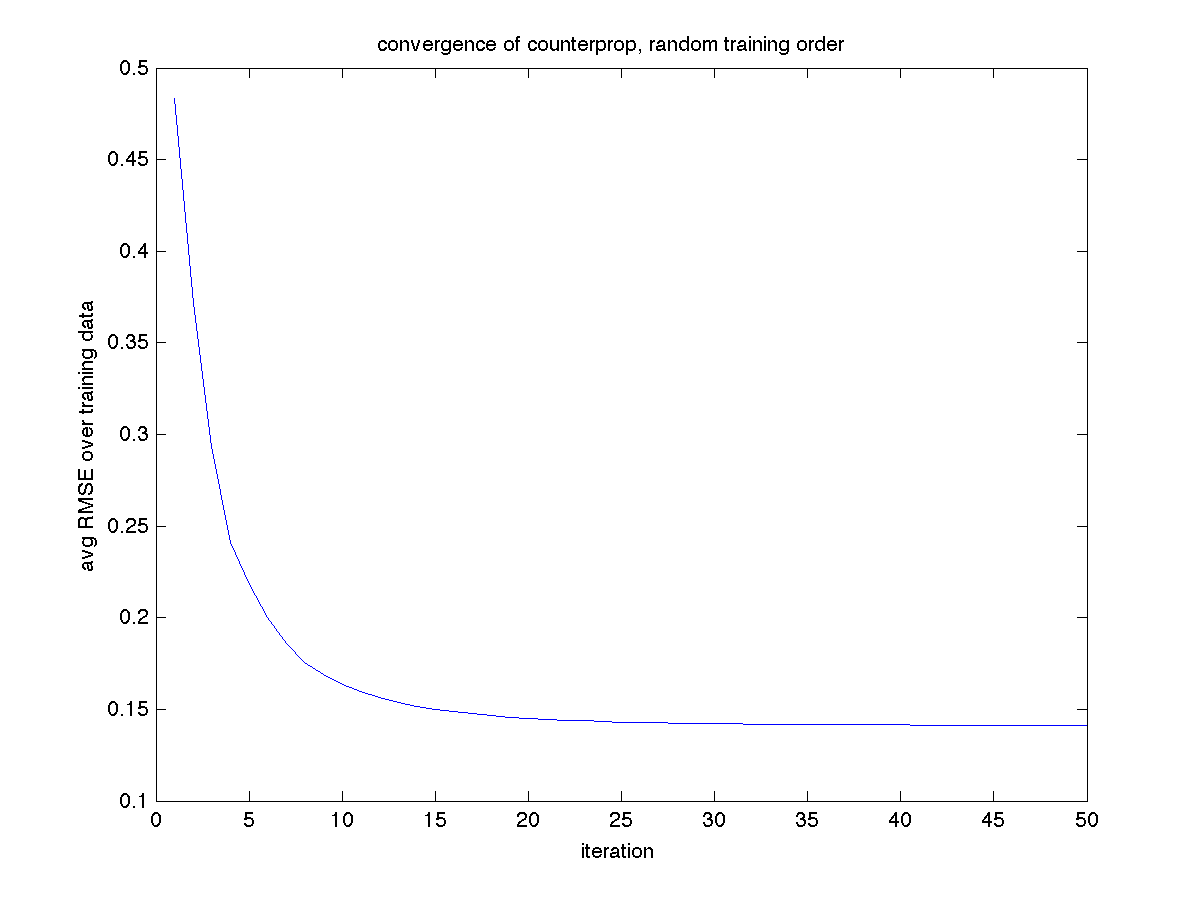
\includegraphics[width=0.68\textwidth]{113.png}
      \label{fig:3}
      \caption{Randomized order of presentation of the training data.}
    \end{figure}

    \begin{figure}
      \centering
      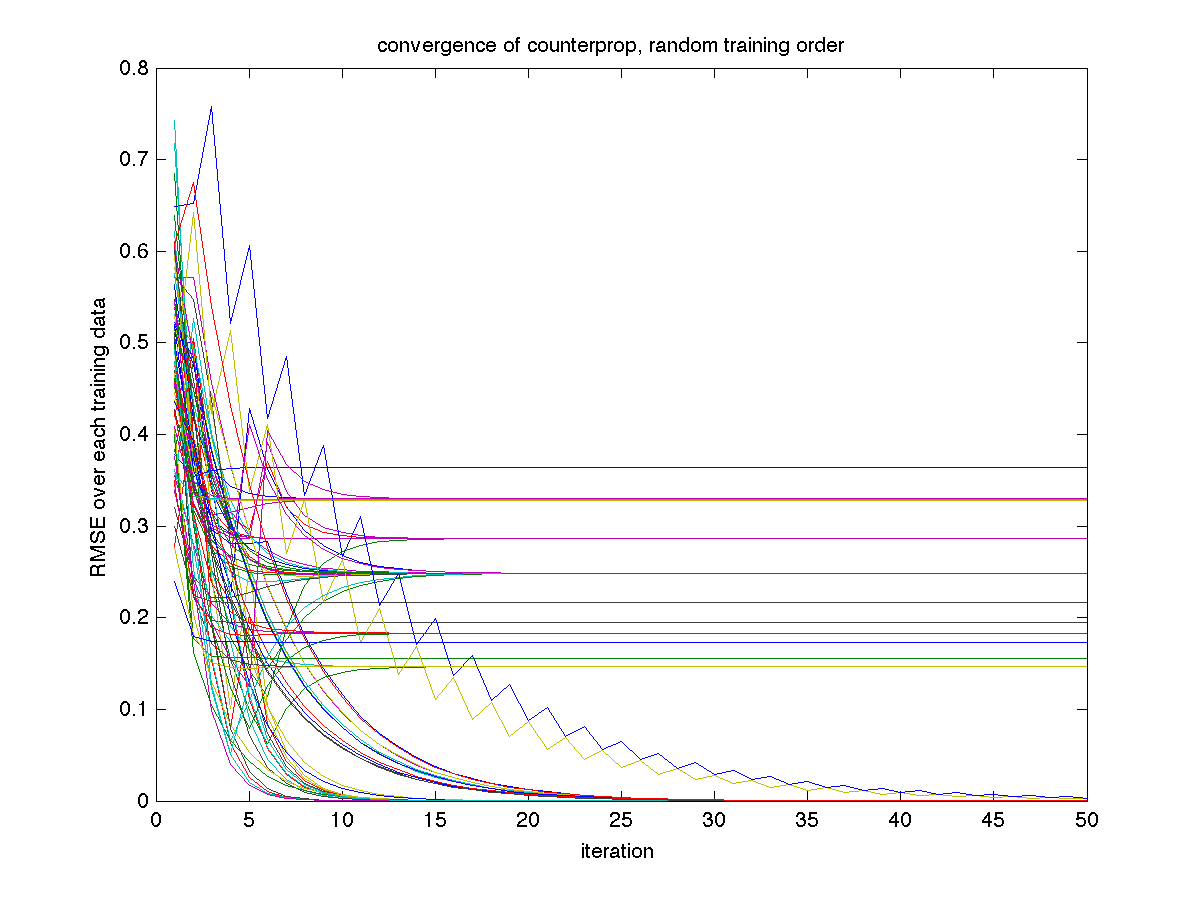
\includegraphics[width=0.68\textwidth]{114.png}
      \label{fig:4}
      \caption{Randomized order of presentation of the training data, and convergence on each of the training data.}
    \end{figure}

    \begin{figure}
      \centering
      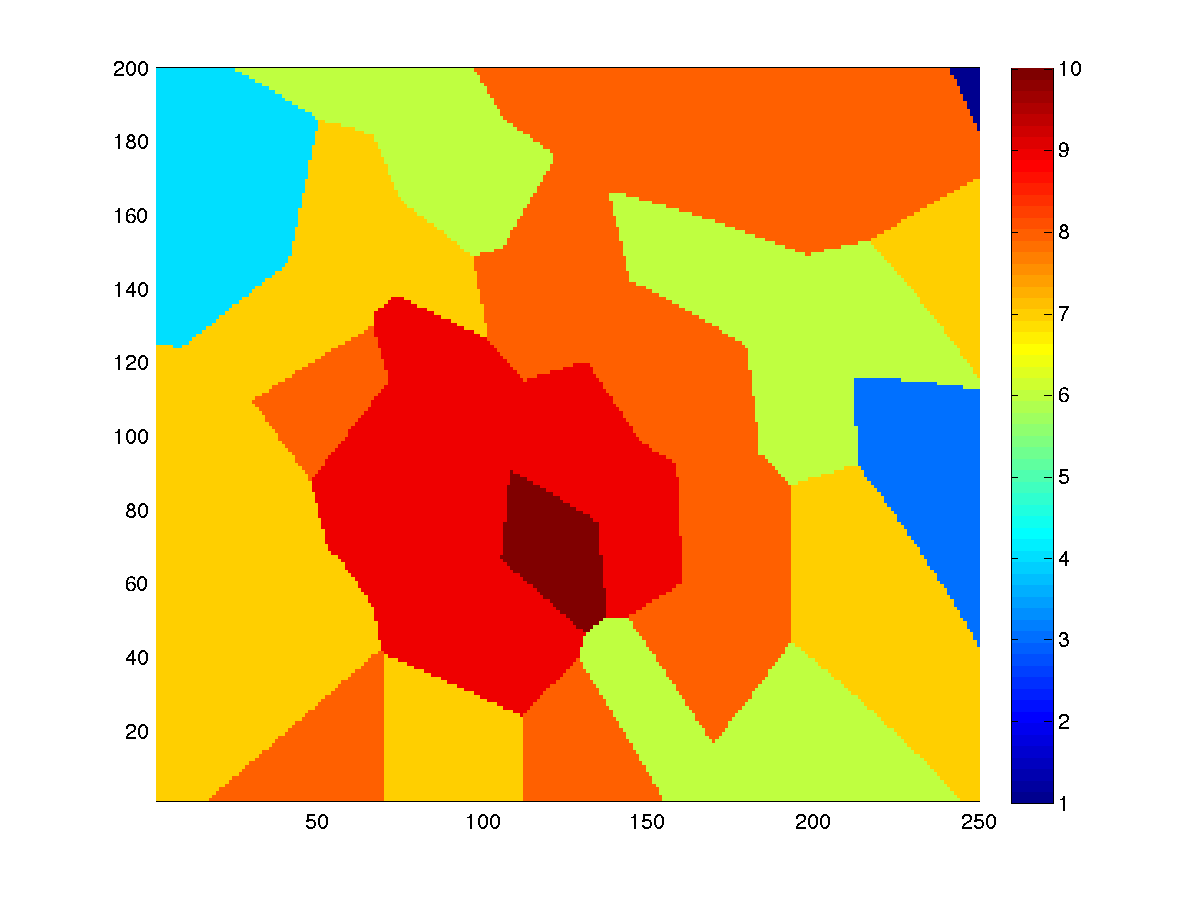
\includegraphics[width=0.68\textwidth]{116-standard.png}
      \label{fig:6}
      \caption{Classification of full data (interpolation phase).}
    \end{figure}

\end{document}
